% entre chaves, adicionar o nome do capítulo.
% o comando \label cria um nome para o capítulo que pode ser utilizado com referência
% cruzada ao longo do texto.

\chapter{Introdução} \label{cap:intro} 

Atualmente existe um grande aumento na frota de motoboys nas cidades devido aos aplicativos de delivery existentes, isto permite ao entregador não ser mais dependente de uma empresa, tornando seu serviço mais acessível e expandindo seu mercado. 

No entanto, os motoboys são os que mais sofrem acidentes. Segundo o Ministério da Saúde, grande parte dos envolvidos são jovens entre 18 e 29 anos de idade nesta categoria (GIANNINI, 2018).

Os aplicativos de delivery mais populares não demonstram preocupações com a saúde de seus colaboradores. Tais aplicativos, apresentando-se apenas como meio mais rápido e barato de realizar os seus serviços, apenas diminuem o tempo de contato entre empresa e entregador como é o caso de Ifood, Rappy e Ubereats. Para tal, este trabalho propõe um aplicativo para ajudar no dia a dia das entregas, capacitado a avisar outros motoboys por perto, através de notificações no dispositivo móvel, em caso de acidente ou necessidade de ajuda, como demonstrado na Figura 1.



\begin{figure}[H]

 \caption{Diagrama simplificado do sistema }
  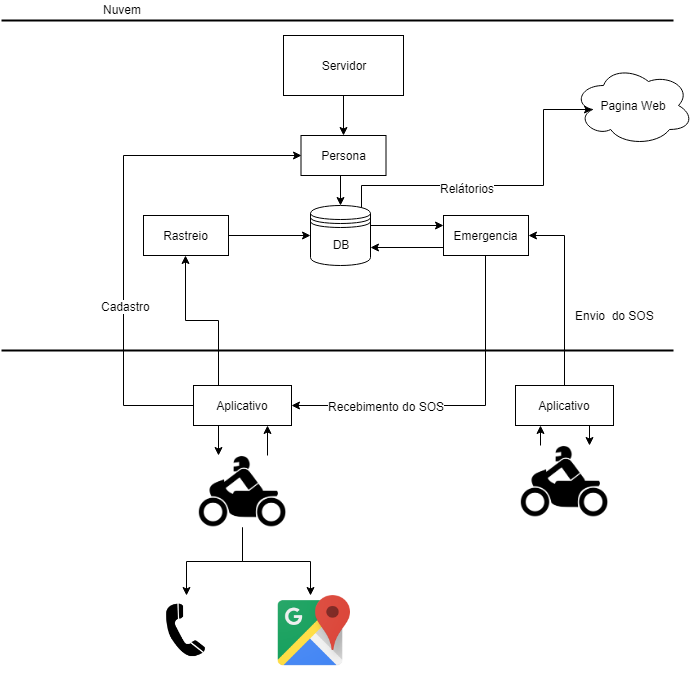
\includegraphics[width=\textwidth]{images/Cap1/tcc.png}
  
  
\end{figure}




O sistema será composto por um hardware fixado na motocicleta, aplicativo para smartphones e um servidor em nuvem.

Para a detecção dos acidentes será utilizado o acelerômetro de três eixos do celular junto com uma placa que também possuirá um acelerômetro externo em um case à prova de impactos e impermeável, possibilitando calcular o ângulo da moto. O hardware e o aplicativo irão comunicar-se através de uma rede wireless para trocar informações e enviar para o servidor.

No aplicativo haverá o registro do motorista, possuindo dados de pessoas próximas para possíveis avisos, além de informações essenciais para identificação da persona. O aplicativo será capaz de redirecionar para os relatórios, contendo as áreas com alta probabilidade de risco de acidentes por período, região além de traçar rotas no Google Maps até a vítima.

O aplicativo irá atualizar a posição do motoboy constantemente para que o sistema possa rastreá-lo corretamente em casos emergenciais. Para isso, o aplicativo ficará monitorando majoritariamente o acelerômetro e possíveis outros sensores do celular.

Quando o aplicativo ou hardware realizar a leitura característica de um possível acidente, será disparado um sinal para o serviço em nuvem, este que alertará os outros motoboys em um raio de distância de 5km. Os alertados poderão ligar para um serviço de emergência, ir até o local, ou falar com algum parente próximo da vítima ou empregador.

Já o servidor será responsável por receber as informações de localização e irá armazenar estes dados dentro de um banco de dados. Estas informações de rastreio serão apagadas depois de um certo período de tempo pois não há necessidade de manter salvo o trajeto de todos os usuários por longos períodos. Com a latitude e longitude do usuário será possível adquirir informações climáticas aumentando a capacidade da análise de dados para futuros relatórios.

Quando o servidor receber um sinal de emergência, ele irá buscar as informações do motorista cadastrados no banco e logo em seguida irá mandar avisos para todos os usuários próximos da região.
Além disso, serão disponibilizados os dados históricos dos eventos ocorridos em formato tabular possibilitando a aplicação de filtros para melhor visualização dos relatórios.



\clearpage
\section{Objetivo Geral}


Desenvolver um sistema emergencial para motoboys, capaz de alertar sobre as áreas com alto risco de acidentes, aviso de pessoas acidentadas na proximidade por meio de notificações, para o serviço emergencial, parentes, empregador ou traçando rota até a vítima.
Junto com isto, será possível apresentar os dados de acidentes em uma plataforma web contendo mapa, condições climáticas, áreas de risco e marcadores possuindo as informações sobre acidentes ocorridos mantendo sigilo da persona envolvida. Também serão disponibilizados os dados históricos dos eventos ocorridos em formato tabular sendo possível aplicar filtros para melhoria da visualização dos relatórios.


\section{Especificação Tecnica}

\begin{enumerate}
    \item Realizar uma pesquisa inicial para determinar o padrão do acelerômetro em caso de acidentes de moto e o tempo de resposta do acelerômetro presente nos smartphones.
\item Verificar necessidade de hardware externo caso o trigger do acelerômetro interno dos smartphones não for suficiente, e, se for verificada esta necessidade, desenvolver este hardware.
\item 	Desenvolver um aplicativo que engloba o cadastro do motorista, suas informações de contato, monitoramento e alerta de acidentes.
\item 	Desenvolver a funcionalidade de relatórios das áreas com maior risco de acidentes.
\item 	Desenvolver Integração do Google Maps para ajuda em criação de rota e análise dos eventos ocorridos.
\item 	Desenvolver as aplicações do servidor permitindo comunicação do app.
\item 	Desenvolver e implementar um esquema para banco de dados estruturado.
\item 	Integrar e testar as aplicações (servidor mais aplicativo).
\item 	Criar uma página web para acesso público dos dados adquiridos.
\item 	Analisar a possibilidade de integração com os aplicativos de delivery existentes.

\end{enumerate}

